%%%%%%%%%%%%%%%%%%%%%%%%%%%%%% -*- Mode: Latex -*- %%%%%%%%%%%%%%%%%%%%%%%%%%%%
%% 10-07-system.tex --  HICSS 44 Kukui Cup paper
%% Author          : Philip Johnson
%% Created On      : Mon Sep 23 11:52:28 2002
%% Last Modified By: Philip Johnson
%% Last Modified On: Mon Jun 14 12:36:48 2010
%%%%%%%%%%%%%%%%%%%%%%%%%%%%%%%%%%%%%%%%%%%%%%%%%%%%%%%%%%%%%%%%%%%%%%%%%%%%%%%
%%   Copyright (C) 2009 Philip Johnson
%%%%%%%%%%%%%%%%%%%%%%%%%%%%%%%%%%%%%%%%%%%%%%%%%%%%%%%%%%%%%%%%%%%%%%%%%%%%%%%
%% 

\section{System Design}
\label{sec:system-design}

\subsection{Requirements}

As our related work findings illustrate, current software for energy
competitions tends to be either commercial, closed systems, or special
purpose, ``one-off'' systems.  We strive in this project to create
software with an architecture that is open, extensible, and easily tailored
to the needs of different universities.  We intend the software
infrastructure from this project to provide as much of a research
contribution as our actual experimental results.

The following general requirements inform our system design.

{\em Open source.}  To maximize the potential for community
participation in development as well as use of the software, we make
all components available as open source, and utilize only freely
available third party components for development.  There are no software
costs associated with the use of our system.

{\em Platform, language, and meter neutrality.}  We want to avoid lock-in
to any particular platform, language, or metering technology.  To avoid
platform lock-in, we develop all components using technologies such as
Java, Python, Javascript, and Google Visualizations that are available on
Windows, Macintosh, and Linux platforms.  To avoid language lock-in, the
system observes a service-oriented architecture, where components
communicate with each other over HTTP via a RESTful API.  This isolates
language dependencies to individual services.  For example, the WattDepot
server is written in Java, while the Makahiki web application framework is
written in Python.  Finally, to avoid metering technology lock-in, the
system architecture involves ``sensors'' that query any given meter using
its native protocol, which then translates the data into a common format for use in
the rest of the system.  Thus, adapting the system to a new meter
technology simply involves implementing the sensor for that technology.

{\em Feature subsetting.} Not all universities need or want the same 
level of sophistication in their dorm energy competitions.  In reviewing 
other sites, we found that they ranged from simple single web pages that are 
edited manually, to advanced sites that integrate near-real time energy data. 
Our software is designed to support users with a variety of needs. 

\subsection{Architecture}

\begin{figure*}[!th]
  \center
  \includegraphics[width=0.8\textwidth]{architecture.eps}
  \caption{\em \small System Architecture: Dorm energy usage is captured by one or more meters, which 
are queried by WattDepot sensors and the raw data sent to the WattDepot server. Analyses are computed
and stored in cloud-based services for ease of retrieval and display in the Makahiki web application.}
  \label{fig:architecture}
\end{figure*} 

Figure \ref{fig:architecture} illustrates the high-level architecture of the
system. There are three basic subsystems in this architecture.  The first is the
dorm electrical infrastructure, illustrated on the left hand side of the
diagram.  This infrastructure includes power distribution to dorm rooms where
residents consume power.  It also includes one or more electrical meters that
monitor power consumption and that are connected to the Internet.  The second
subsystem is WattDepot, an open source suite of tools for enterprise-level
collection, storage, analysis, and presentation of energy data
\cite{Brewer2010WattDepot, WattDepot}. The third subsystem is Makahiki, an open source
framework for building dorm energy competition web applications. The following
sections discuss each of these architectural components in more detail.

\subsubsection{WattDepot Sensors}

In order to track energy consumption or production, a physical meter of some
sort is required. Energy meters come in a variety of designs from many
manufacturers, and the manufacturers often provide some sort of management
or data collection software. However, the data collection software is often
closely tied to a particular brand of device, making data collection from
heterogeneous meters complicated and reducing flexibility when selecting a
meter vendor.

WattDepot solves this problem through the introduction of software ``sensors''
that collect data from a type of meter and send that data in a standardized
format to a WattDepot server using the Internet and the RESTful WattDepot API
over HTTP. This encapsulates the meter-specific code into the sensor, allowing
meter selection to be performed independent of storage, analysis, and
visualization capabilities.

\subsubsection{WattDepot Server}
\label{sec:wattdepot-server}

The WattDepot server acts as the central hub for energy data: sensors send
energy data to the server, and clients make requests to retrieve data from the
server for analysis or visualization. To allow for flexibility and
extensibility, the server provides a RESTful web services API. REST
(REpresentational State Transfer) \cite{REST} is a specification paradigm,
which, when applied to web services, generally results in more easily usable and
extensible communication than alternatives such as SOAP. The WattDepot API
\cite{WattDepotAPI} provides more details and a full specification of the
supported operations.

Two other notable features of the WattDepot server are meter aggregation and
data interpolation. When deploying meters to monitor a large installation such
as a building, it may require multiple meters to track the energy usage of a
single logical unit, such as floor of a building. WattDepot allows the
specification of virtual sources that aggregate the energy data from all their
sub-sources. These virtual sources make it easier for clients to retrieve
data about logical units (such as floors) without having to worry about the
details of the meter installation.

When multiple meters are used to monitor a single logical unit, another common
issue is the ``timestamp problem''. The internal clocks on meters may not be
synchronized, and interval between successive queries of meter data by a sensor
may not be uniform. This can lead to a virtual source that aggregates meter data
from two subsources where the timestamps of the energy data differ
significantly. Clients will often want to request energy data from a virtual
source at an arbitrary time, independent of the data timestamps the server
actually possesses. WattDepot solves this problem by linearly interpolating
energy data requests from clients that lie between timestamps of recorded meter
data. This allows the energy data retrieved from meters to be stored verbatim,
while allowing clients the flexibility to request data at arbitrary times.
If the energy data is being sampled frequently, the error from interpolation
should be relatively low.

\subsubsection{WattDepot Cloud Cache}

A typical dorm energy competition will involve hundreds to thousands of
students.  Energy data requests are characterized by the desire for
relatively recent results. For example, how much power did my dorm use in
the last hour, and how does that compare to usage during the same hour over
the past month? They are also characterized by the fact that those same
results do not tend to be user-specific: monitoring the energy usage of
individual dorm members is not practical at the current time; the most
fine-grained collection we have seen is floor-level. These two application
characteristics argue for caching of results so that the WattDepot server
is not processing the same request hundreds or thousands of times.

The architectural issue is: where should that cache of reusable data be
placed?  There are three choices: in the server, in the web application, or
in a third service ``in between'' the server and the web application.
All of these approaches have their strengths and weaknesses.  Our system
architecture chooses the last approach, in which a service called
WattDepot-GData creates Google Docs spreadsheets containing high level
abstractions of the raw data stored in the WattDepot server.  We chose the
Google Docs cloud-based storage system because it is free, it is scalable
and very high performance, and it integrates extremely well with the Google
Visualization API.  This latter feature enables the Makahiki web
application framework to provide advanced, interactive visualizations of
energy data with very little end-user coding.

\subsubsection{Makahiki}

\begin{figure*}[htbp]
  \center
  \includegraphics[width=0.8\textwidth]{makahiki.eps}
  \caption{\em \small An example dorm energy web application built with Makahiki.}
  \label{fig:makahiki}
\end{figure*} 

The final subsystem in our architecture is called Makahiki \cite{makahiki-site}, which is a
framework for developing dorm energy competition web applications.  Figure
\ref{fig:makahiki} illustrates the home page for the University of Hawai`i
dorm energy web application built as a configuration of Makahiki. As a
framework, Makahiki supports several forms of tailoring without requiring
any editing of the underlying Python source code.

{\em Configurable look and feel.} The color scheme and logos for the site
are defined in CSS files that can be edited or replaced to best reflect the
University's color scheme. At the University of Hawai`i, Makahiki is
configured with a green and white color scheme and the ``Kukui Cup'' name
and logo.   We use the JQuery ThemeRoller application to simplify the generation of 
alternative look and feels.

{\em Configurable display panes.} Each page in the web application generated by Makahiki
contains a number of display panes. The contents of these display panes can be easily 
reconfigured. For example, the form of energy visualization can be changed by editing 
the underlying Javascript associated with the display pane. 

{\em Configurable functional modes.}  Makahiki supports several functional ``modes'', which 
enable it to conform to the needs of a wide variety of dorm energy competitions.  

The ``single page'' mode is the simplest mode, which enables a university
to create a simple, single page website with a matching look and feel for
their university.  In single page mode, energy data and dorm standings can
be visualized by manually creating Google Docs spreadsheets and configuring
the display panes to visualize the data as tables or bar charts.  In this
basic functional mode, there need not be any use of WattDepot; all data can
be collected manually by competition organizers and entered into
spreadsheets for display.

In ``multi page'' mode, Makahiki generates a web application containing a
Home page, a Resources page, an Energy data page, a Competition page, and
an About page.  Multi page mode provides a more comprehensive web
application that enables the university to provide significantly more
information than is possible with single page mode.  As with single page
mode, multi page mode does not require WattDepot.

The final mode is called ``login'' mode, and it is in this mode that
Makahiki provides features not currently found in other dorm energy
competition web applications.  In this mode, each resident of the dorm can
login (using their university-assigned credentials) to their own personally
customized home page, which provides access to energy data regarding their
floor as well as behavioral change tools. Login mode requires automated access
to energy data and so WattDepot is required.  Figure \ref{fig:makahiki-login}
illustrates a sample configuration of an individual user home page.

\begin{figure*}[htbp]
  \center
  \includegraphics[width=0.8\textwidth]{makahiki.login.eps}
  \caption{\em \small The personalized user home page with floor-level monitoring and behavioral change tools 
including commitments, activities, and goals.}
  \label{fig:makahiki-login}
\end{figure*} 

The design of Makahiki's login mode is based upon research findings
regarding behavioral change in energy consumption, which indicate that
feedback, commitments, goal setting, knowledge, and incentives are all
important mechanisms to create sustained change.  Makahiki provides
feedback regarding energy usage via near-real time data on the user's
floor's cumulative energy usage during the competition, instantaneous power
consumption, and comparisons to baseline measures and other
floors. Activities are individual, concrete actions such as attending a
meeting or movie showing about energy, watching an energy-related video, or
reading news articles, all of which are designed to heighten the student's
knowledge and awareness of energy. Commitments are more general changes in
behavior, such as turning off the lights when leaving any room.  Finally,
goals are behaviors involving the floor as a whole, such as attempting to
reduce energy usage by 10\% over the next week. The weekly energy reduction
goal is picked collaboratively by the group participants through voting, and
progress towards the goal is visualized with a variety of charts.

To incentivize participation in activities, goals, and commitments,
Makahiki provides the capability for users to accumulate points for
completing instances of these three types of actions.  Makahiki supports
verification of activities and goals. When defining an activity for
inclusion in the system (such as the watching of a short YouTube video on
wind energy), the site administrator also can enter several short questions
whose answers are found in the video (such as ``What is the average power
output of the wind turbine in the video?'').  When a user requests to
receive points for having performed that activity, the system will prompt
the user with a question selected at random.  The user's request, with
their answer, is reviewed by administrators who can decide whether or not
to confirm or deny the request.  

Commitments, while an important tool for behavioral change, are problematic
to verify.  Makahiki addresses this issue in several ways.  First,
commitments are worth less points than verifiable activities or goals.
Second, commitments are active for a period of five days, and when the user
requests points at the end of that time, they must self-verify that they
satisfied the commitment.  Finally, and most importantly, commitments are
public: the Makahiki website broadcasts the commitments entered into by the
users. Research shows that making public commitments are a powerful incentive
for behavioral change.

To leverage students' use of social networking sites, Makahiki will
integrate with Facebook. With the consent of the participant, Makahiki will be
able to post messages to the participant's ``wall'' when they make commitments,
or complete activities. Facebook integration is expected to increase the
visibility of the competition, and encourage the participant's peer group to
engage in the competition.

Mobile phones capable of running applications and browsing the web are an
increasing part of college students' information ecosystem. To make it as easy
as possible for residents to participate, we are developing a version of the
Makahiki website optimized for mobile phones. The mobile-optimized website will
provide the essential functions: displaying energy usage and contest standings,
progress towards goals, and completion of activities.

Another way to keep residents aware of the competition is an electronic
billboard displayed in the lobby of the dorms. The billboard rotates through a
variety of competition information, such as upcoming events, recent commitments,
energy usage, and competition standings. The billboard is being implemented as
a single web page with embedded JavaScript, which queries the WattDepot Cloud
Cache for energy data and Makahiki for competition data. The web page can be
displayed to residents using a large television connected to a networked
computer. The billboard is assembled using the open data and components of
WattDepot and Makahiki, making future extension possible.